\documentclass{article}
\usepackage[legalpaper, margin=1in]{geometry}
\usepackage{amsmath}
\usepackage{algorithm}
\usepackage[noend]{algpseudocode}
\usepackage{graphicx}
\usepackage{amssymb}
\usepackage{scrextend}
\usepackage{indentfirst}
\usepackage{caption}
\usepackage{subcaption}
\graphicspath{ {./images/} }
\DeclareMathAlphabet{\mathcal}{OMS}{cmsy}{m}{n}
\SetMathAlphabet{\mathcal}{bold}{OMS}{cmsy}{b}{n}
\begin{document}

\begin{flushright}
William Tidwell \par
gtg004s \par
CS8803 - Adaptive Control and Reinforcement Learning \par
\today \par
\end{flushright}

\begin{center}
Assignment 1
\end{center}

\begin{flushleft}
a) Discussed with: Pol Llado\par
b) Sources: Textbooks and TA Office Hours \par
\end{flushleft}

\section{Initialization}
The purpose of this assignment is to gain a better understanding of Linear Quadratic Regulators (LQR) by designing a controller for an unstable robot. A model that simulates an XCell Tempest helicopter in the flight regime close to hover is used for the exercise. 

We start of by running the helicopter in open-loop, starting from the trim state. The NED plot is shown below. We can see that the position remains constant for all dimensions.

\begin{figure}[h]
\centering
\begin{subfigure}{.5\textwidth}
  \centering
  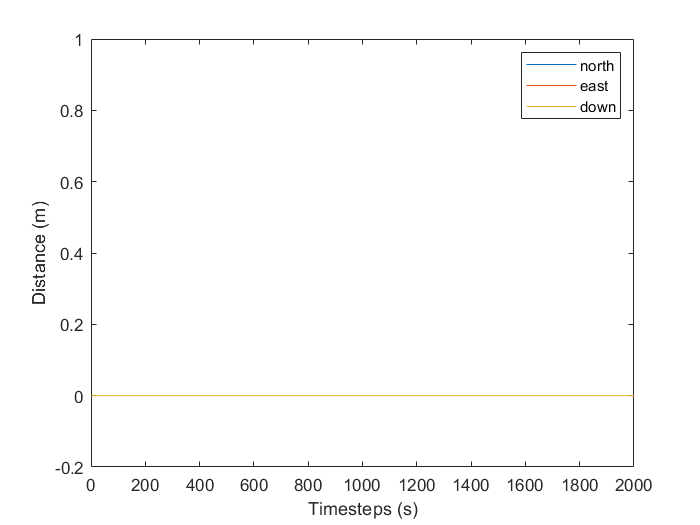
\includegraphics[width=.95\linewidth]{open_loop}
  \caption{Without Noise}
  \label{fig:sub1}
\end{subfigure}%
\begin{subfigure}{.5\textwidth}
  \centering
  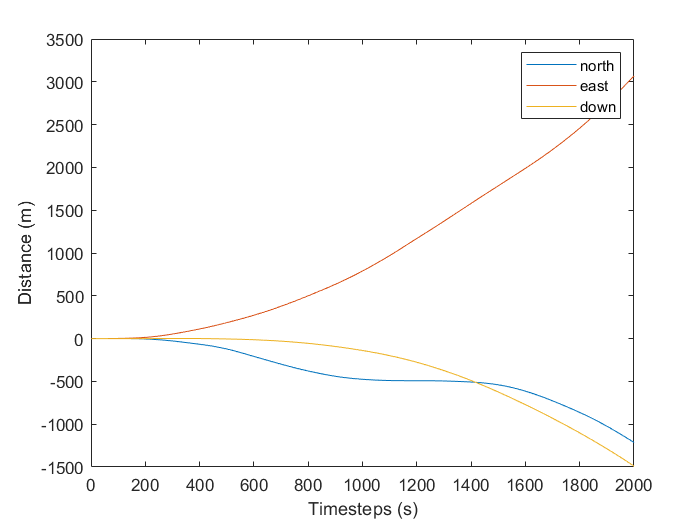
\includegraphics[width=.95\linewidth]{open_loop_noise}
  \caption{With Noise}
  \label{fig:sub2}
\end{subfigure}
\caption{Open Loop NED Plots}
\label{fig:test}
\end{figure}

% \begin{figure}[h]
% \caption{Open Loop NED}
% 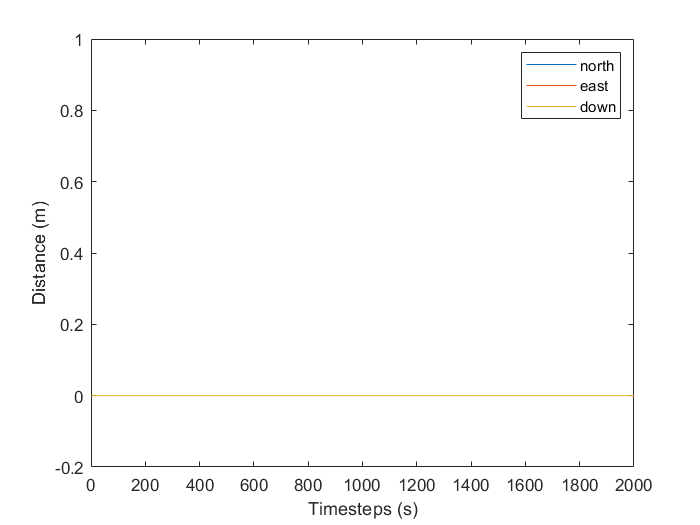
\includegraphics[width=0.75\textwidth]{open_loop}
% \centering
% \end{figure}

Next, we add some noise to the simulation and examine the NED plot. It becomes immediately evident that the helicopter very quickly diverges from the desired hover state.

% \begin{figure}[h]
% \caption{Open Loop with Noise NED}
% 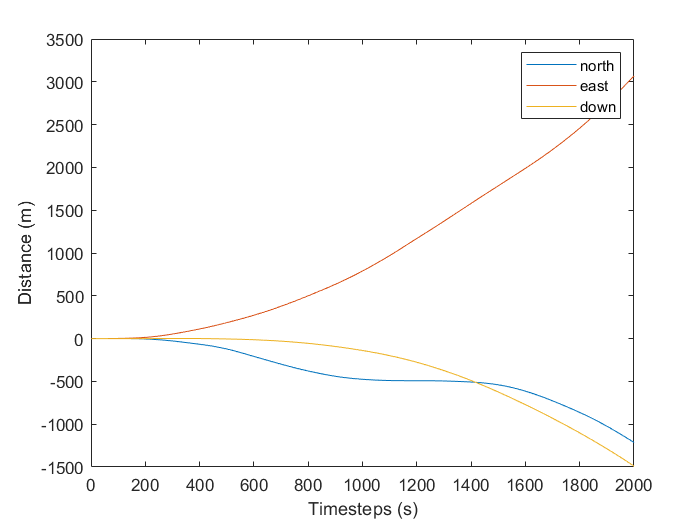
\includegraphics[width=0.75\textwidth]{open_loop_noise}
% \centering
% \end{figure}

\section{Steady State LQR Controller}

 The first task is to design a steady state LQR controller. Given states $x$, we can use the controller $k$ to find a corresponding set of actions $a$ with the following relationship

\begin{align}
    u_t = k_t x_t
\end{align}

The goal is to find a value of $k$ once the system has stabilized and is running at steady state. We will call this value $k_{ss}$. The algorithm outlined below can be used to find $k_{ss}$.

\begin{algorithm}
\begin{algorithmic}[1]
\Function{k-ss}{A, B, Q, R, T}
	\State $P \gets Q$
	\For {$i \gets 1:T$}
		\State $k(i) \gets -(B^T P B + R)^{-1} B^T P A$
		\State $P \gets Q + k(i)^T R k(i) + (A + B k(i))^T P (A + B k(i))$
	\EndFor
	\State \Return $k(T)$
\EndFunction
\end{algorithmic}
\end{algorithm}

where $A$ and $B$ are used to represent the dynamics in the form

\begin{align}
    x_{t+1} = Ax_t + Bu_t
\end{align}

$Q$ and $R$ are used to calculate the quadratic cost as

\begin{align}
    c(x, u) = x^TQX + u^TRu
\end{align}

and $T$ represents the horizon, or number of timesteps the algorithm runs. The plot below shows the convergence of all K-values. The values seem to have converged after around 100 iterations, and the search could have been terminated much earlier than it was. 

% \begin{figure}[h]
% \caption{Convergence of K Values}
% 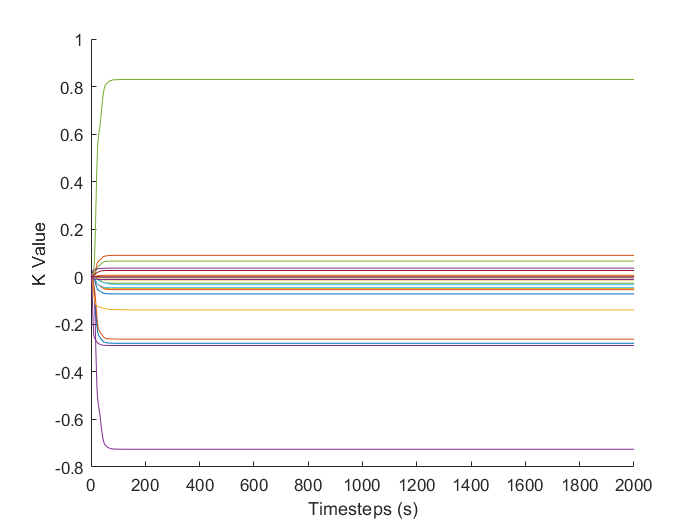
\includegraphics[width=0.75\textwidth]{k_convergence}
% \centering
% \end{figure}

The NED plot using the new controller can be seen below, and it looks identical to the Open Loop NED plot from above. This indicates that the controller is at least capable of keeping the helicoper hovering in the desired position under perfect conditions.

\begin{figure}[h]
\centering
\begin{subfigure}{.5\textwidth}
  \centering
  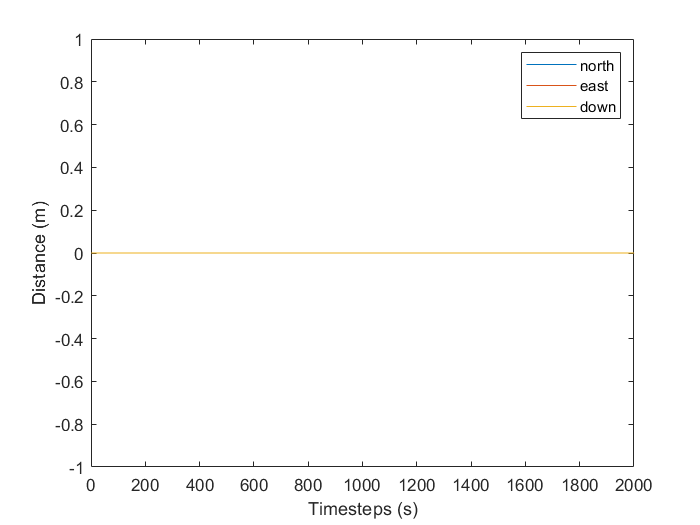
\includegraphics[width=.4\linewidth]{kss_hover}
  \caption{A subfigure}
  \label{fig:sub1}
\end{subfigure}%
\begin{subfigure}{.5\textwidth}
  \centering
  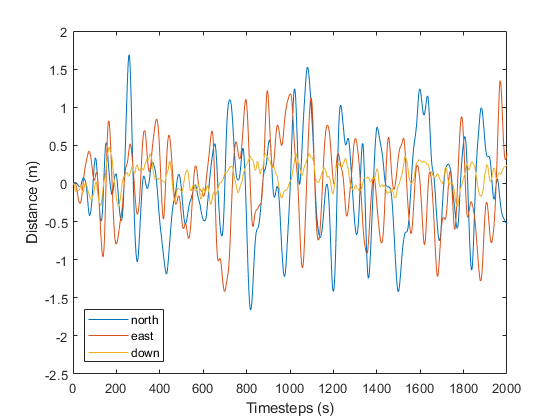
\includegraphics[width=.3\linewidth]{kss_hover_noise}
  \caption{A subfigure}
  \label{fig:sub2}
\end{subfigure}
\caption{A figure with two subfigures}
\label{fig:test}
\end{figure}

% \begin{figure}[h]
% \caption{$K_{ss}$ Hover NED}
% 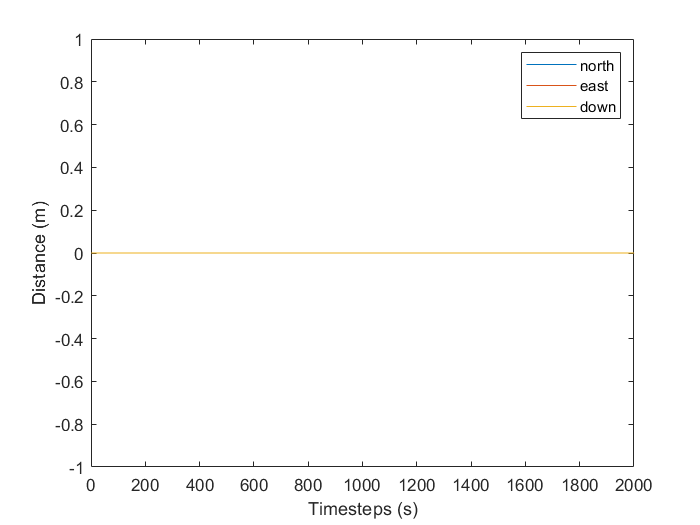
\includegraphics[width=0.5\textwidth]{kss_hover}
% %\centering
% \end{figure}

Next we test the controller by adding noise to the simulation. 

% \begin{figure}[h]
% \caption{$K_{ss}$ Hover with Noise NED}
% 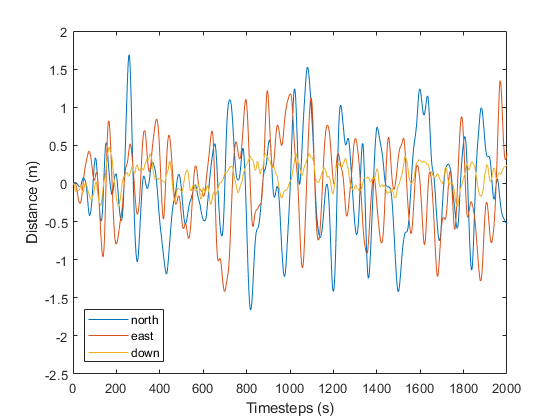
\includegraphics[width=0.5\textwidth]{kss_hover_noise}
% %\centering
% \end{figure}


Problem: Suppose we have: $n$ cities, $C = \{c_1, c_2, ..., c_n\}$, $m$ roads, $R = \{r_1, r_2,..., r_m\}$, each connecting a pair of cities; and a constant $k \in \{2,...,|C|-1\}$. If we are given a subset $T$ of roads, $T \subseteq R$, then define $d_T(u)$ as the number of roads that city $u$ is connected to using only roads in $T$. We want to find a subset $T$ such that $|T| \leq |C|-1$ such that $1 \leq d_T(u) \leq k$ for all nodes $u \subseteq C$, and all cities in $C$ are connected together. We will call this the Fiber Connectivity problem, and we will denote it with the symbol $Y$.\\

This problem sounds very similar to a special case of the Hamiltonian Path problem. A Hamiltonian Path is a path between two vertices that visits every other vertex in the graph exactly once. \\

Step 1: Show that the Fiber Connectivity problem is in NP. \\
Certificate: A subset $T$ and the original graph $G=(V,E)$ where $V$ is the set of cities and $E$ is the set of roads. \\
Certifier: Verify that $T \subseteq R$ (linear), $|T| \leq |C|-1$ (linear), $1 \leq d_T(h) \leq k$ for all nodes $u \subseteq C$, and all cities in $C$ are connected together ($\mathcal{O}(V+E)$.\\

Step 2: Choose Hamiltonian Path as NP-Complete problem, and denote it with the symbol $X$. \\

Step 3: Prove that $X \leq_p Y$ and show that $X(i) = YES \Leftrightarrow Y(f(i))= YES$. \\
Lemma: Given a graph $G=(V,E)$, $G$ contains a Hamiltonian Path iff $G$ contains a Fiber Connectivity with $k=2$.
Proof: Let $X \subseteq E$ be a Hamiltonian Path of size $|V|-1$ in $G$. Then $Y \equiv E$ is a Fiber Connectivity where $k=2$ in $G$. \\
Reduction: For the reduction, the same graph $G$ can be used in both instances. We need pass the parameter $k=2$ to the Fiber Connectivity problem.\\

Case 1: $X(i)$ is a yes instance. \\
Let $P \subseteq E$ be a solution to the Hamiltonian Path problem. We know that $|P|<|V|-1$, and every node $v \in V$ is in $P$. For the sake of contradiction, assume that $P$ is not a solution to the Fiber Connectivity problem with $k=2$. There are a few conditions that must be satisfied to be a Fiber Connection: $|P| \leq |V|-1$, $1 \leq d_T(u) \leq 2$ for all nodes $u \subseteq V$, and all nodes in $V$ are connected together. But by the definition of a Hamiltonian Path, $|P| \leq |V|-1$, all nodes are visited exactly once, so $1 \leq d_T(u) \leq 2$ for all nodes $u \subseteq V$, and since it is a path, all nodes are connected. Thus $P$ must be a solution to the Fiber Connectivity Problem.\\

Case 2: $Y(f(i))$ is a yes instance. \\
Let $T \in E$ be a solution to the Fiber Connectivity Problem with $k=2$. For the sake of contradiction, assume that $T$ is not a solution to the Hamiltonian Path problem. We know that $|T|<|V|-1$, that $1 \leq d_T(u) \leq 2$ for all nodes $u \subseteq V$, and that all nodes are connected. This means that $T$ is path connecting all nodes, and no node is visited more than once. This is the definition of a Hamiltonian Path, so we have a contradiction.

\newpage
\section{Minimum Set Cover}

\subsection{}

a) The subproblem is the remaining unassigned subsets that can be included in a partial solution.\\

b) We choose a subproblem to expand based on how promising it looks, or how likely it seems to produce a good or even optimal solution. Usually some sort of scoring metric is used to evaluate a partial solution, and this scoring metric is the priority used in the priority queue or frontier set of configurations. The lower bound is one such metric and is frequently used.\\

c) The general formula is to consider all candidate extensions i.e. all remaining subproblems. For each remaining subproblem, we first check to see if it including it generates a solution. If so, and if the solutions cost is better than the current best cost, we update the best cost and save the solution. If no solution is found, and the candidate does not create a dead-end, a lower bound is calculated for the new partial solution. If the lower bound looks promising, meaning it is less than the current best cost, then it is added to the frontier set of configurations. For the Set Cover problem, we would consider adding each unassigned subset to the current partial solution and evaluating based on the steps outlined above. \\

d) An appropriate lower bound could be the number of subsets comprising the partial solution. If it is already higher than the number of subsets needed for the current optimal solution, the partial solution can be discarded. For a tighter bound, one could also consider the sizes of the unassigned subsets and add the minimum number of subsets possible to obtain a solution to the number of subsets already used. For example, if 5 elements remain to be covered, and all subsets are of size 3, then add 2 to the current number of subsets in the partial solution.\\

\begin{algorithm}
\begin{algorithmic}[1]
\Function{Set-Cover-Lower-Bound}{U, soln, options}
	\State sort $options$ by length of subsets in nondecreasing order
	\State $numCovered \gets $ length of set of all elements in $soln$
	\State $lb \gets soln.length$
	\State $i = 0$
	\While {$numCovered < U.length$}
		\State $numCovered \gets numCovered + options[i].length$
		\State $lb \gets lb + 1$
	\EndWhile
	\State \Return $lb$
\EndFunction
\end{algorithmic}
\end{algorithm}

\begin{algorithm}
\begin{algorithmic}[1]
\Function{Set-Cover-Branch-and-Bound}{U, S}
	\State $optSoln \gets$ Array[]
	\State $minK \gets \infty$
	\State $f = $ PriorityQueue()
	\For {each $S_i$ in $S$}
		\State $options \gets S - S_i$
		\State $f.push((0, 1, S_i, options))$
	\EndFor
	\While {$f$ not empty}
		\State $currPriority, currK, currSoln, currOptions = f.pop()$
		\For {each $option$ in $currOptions$}
			\State $newSoln \gets currSoln.append(option)$
			\State $newK \gets currK + 1$
			\If {isSolution($newSoln$) and $newK < minK$}
				\State $optSoln \gets newSoln$
				\State $minK \gets newK$
			\Else
				\State $newOptions \gets currOptions - option$
				\State $lb \gets $ lowerBound($U, newSoln, newOptions$)
				\If {$lb < minK$}
					\State $f.push((lb, newK, newSoln, newOptions))$
				\EndIf
			\EndIf
		\EndFor
	\EndWhile
	\State \Return $optSoln, minK$
\EndFunction
\end{algorithmic}
\end{algorithm}

\subsection{}

To develop a Greedy Algorithm for the Set Cover problem, we first assign a weight $w_i \geq 0$ to each subset $S_i$. The goal is the find a Set Cover $C$ that minimizes $\sum_{S_i \in C} w_i$. The Greedy Algorithm will build the solution one set at a time. To choose the next set, it looks for sets that have small weight $w_i$ and cover many elements. To do so, it uses the ratio $w_i/|S_i|$, which gives a cost per element to cover each element in $S_i$. After some sets have been selected, we are only interested in choosing elements that remained uncovered. A set $R$ is used to track these elements, and the selection criteria is updated as $w_i/|S_i \cap R|$. The algorithm will generate a set cover, but we need to determine how much larger this is than the optimal, $w*$. We will start by defining $c_s = w_i/|S_i \cap R| for all s \in S_i \cap R$. As each set $S_i$ is selected, its weight is distributed over the elements and accounted for in its cost $c_i$. If $C$ is the set cover obtained by the Greedy Algorithm, then we can say $\sum_{S_i \in C} w_i = \sum_{s \in U} c_s$. We need to determine how much total cost any single set $S_k$ can account for by giving a bound to $\sum_{s \in S_k} c_s$ relative to the weight $w_k$. We can us the following ratio $$\frac{\sum_{s \in S_k} c_s}{w_k}$$ Next we need to use the Harmonic Function $$H(n)=\sum_{i=1}^{n} \frac{1}{i}$$ From the definition of the harmonic function, it can be shown that $H(n)=\Theta(\ln n)$, which gives an upper bound on the Greedy Set Cover algorithm.

\subsection{}

a) We are trying to find all $n$ elements with the fewest subsets $m$ possible, so I would consider a scoring function that takes both of those into account. If using a priority queue that prioritizes smaller values, perhaps $m / n$. This way, with two partial solutions both containing $n-x$ elements, the one made up of fewer subsets will be given higher priority.\\

b) The neighborhood would be all subsets, where I could swap subsets from my partial solution with subsets not yet used. The size of the neighborhood would be $\mathcal{O}(n)$. Depending on the size of the problem, this could be refined to say that only subsets containing uncovered elements are considered neighbors. The theoretical complexity doesn't change, but the practical implementation could be much improved.\\

c) Tabu Memory helps avoid comparing the same two subsets for swapping very close together. If a pair has recently been analyzed, it doesn't make sense to compare them again shortly thereafter. I would store $m$ comparison, where each comparison is made up of a subset in the partial solution and a subset in the unassigned subsets. The size of the Tabu Memory, $m$, would depend on the size of the problem and would need to be experimented with to determine optimality.

\newpage
\section{Optimizing Amazon's Operations}

\subsection{}

a) A subproblem here is the possible locations where warehouses can be built but have not yet been considered.\\

b) We want to choose subproblems based on how promising they look, or how likely they are to produce a better solution than the current best. In this case, we want to choose subproblems that we think will minimize our objective function, which is the sum of the costs to build the warehouses and the sum of the minimum distances from each city to a warehouse.\\

c) The algorithm expands the subproblem by looking at all possible options that could be added to the partial solution. \\

d) I found the lower bound for this problem to be rather difficult to define. A very naive option is the set the lower bound to zero. However, this somewhat defeats the purpose of the branch-and-bound, as not many branches can be pruned in this way! I also considered taking the lower bound to be the sum of the costs of the warehouses in the partial solution. If this sum is greater than the current best cost, then it can be discarded. However, depending on what units are used for distance and cost, one could very easily encounter a problem where distances are much greater than building costs, and therefore the contribution of the warehouse cost to the total cost would be small, making the lower bound not much better than zero. I eventually decided to use only the sum of the minimum distances to each warehouse in the partial solution over using the warehouse costs. If we were to set the costs to build warehouses to zero, the objective function would become to minimize the sum of the distances. By ignoring the warehouses, we can focus on reducing the distance. As long as the total distance is less than our current best cost, we can consider a partial solution.\\

\begin{algorithm}
\begin{algorithmic}[1]
\Function{Warehouse-Lower-Bound}{partialSoln, cities, buildCosts}
	\State $totalDistance \gets 0$
	\For {each $city$ in $cities$}
		\State $distance \gets \infty$
		\For {each $warehouse$ in $parialSoln$}
			\If {$d(warehouse, city) < distance$}
				\State $distance \gets d(warehouse, city)$
			\EndIf
		\EndFor
		\State $totalDistance \gets totalDistance + distance$
	\EndFor
	\State \Return $totalDistance$
\EndFunction
\end{algorithmic}
\end{algorithm}

\begin{algorithm}
\begin{algorithmic}[1]
\Function{Warehouse-Branch-and-Bound}{warehouses, cities, buildCosts}
	\State $optSoln \gets $Array[]
	\State $minCost \gets \infty$
	\State f = PriorityQueue()
	\For {each $warehouse$ in $warehouses$}
		\State $cost \gets$ calcCost($[warehouse], cities, buildcosts$)
		\If {$cost < minCost$}
			\State $minCost \gets cost$
			\State $optSoln \gets [warehouse]$
		\EndIf
		\State $f.push((cost, cost, [warehouse], warehouses - warehouse))$
	\EndFor
	\While {$f$ not empty}
		\State $priority, currCost, currSoln, currOptions = f.pop()$
		\For {each $option$ in $currOptions$}
			\State $newSoln \gets currSoln.append(option)$
			\State $newCost \gets \text{calcCost}(newSoln, cities, buildCosts)$
			\If {$newCost < minCost$}
				\State $optSoln \gets newSoln$
				\State $minCost \gets newCost$
			\Else
				\State $newOptions \gets currOptions - option$
				\State $lb \gets $ lowerBound$(newSoln, cities, buildCosts)$
				\If {$lb < minCost$}
					\State $f.push((lb, newCost, newSoln, newOptions))$
				\EndIf
			\EndIf
		\EndFor
	\EndWhile
	\State \Return $optSoln, minCost$
\EndFunction
\end{algorithmic}
\end{algorithm}

\subsection{}

A simple Greedy approach can be defined as follows. First, we will add a restriction that any warehouse will be built in one of the cities. This helps reduce the problem size. Then, we repeatedly choose the next location for the warehouse as the city that is farthest from any existing warehouse. Repeat until $k$ warehouses have been placed. In our case, since we do not have the number of warehouses specified, we would need to repeat for all $k$ from $1,...,n$. Running the algorithm once through has a complexity of $\mathcal{0}(km)$ where $m$ is the number of cities. Since we need to do this for all $n$, we have $T(n) = m\sum_{i=1}^{n}i$, or $T(n)=\frac{mn(n-1)}{2}$, which gives a complexity of $\mathcal{O}(n^2)$. For the analysis, we can define $r(W)=max_i dist(s_i, W)$ as the smallest covering radius, which is the largest distance from any city to its closest warehouse. Let $W*$ be an optimal set of warehouses. Then $r(W) \leq 2r(W*)$. We know that any two centers are at least $r(W)$ distance apart. We can say that $dist(W_i, W*_i) \leq r(W*) < 1/2 r(W)$, so at least one $W*_i$ in each circle of radius $1/2 r(W)$ from each $W_i$. This means the Greedy approach is a 2-approximation.

\subsection{}

a) A possible scoring function would be the total cost $$\sum_{i \in W} f_i + \sum_{j \in \{1,...,m\}} \min_{i \in W} d(i, j)$$ as defined in the problem defintion.\\

b) The neighborhood could be all locations not currently included in set $W$. However, one could also considering simply adding a location to $W$ or removing a location from $W$. Since the optimal size of $W$ is not known, all possibilities need to be considered. In all cases, the neighborhood is on the order of $\mathcal{O}(n)$, where $n$ is the number of locations.\\

c) Similar to the Minimum Set Cover problem above, Tabu Memory is used to avoid trying the modifications to the partial solution multiple times very close together. For this problem, I would store the operation performed and which node(s) were included. For example, if I had recently added/removed a node and the solution quality improved, it might not make sense to immediately remove/add it again. Similarly, if a pair of nodes had recently been swapped, we might need to wait a while until the partial solution has changed before attempting the same swap again.\\

\end{document}